\section{Accuracy estimation with Microprofiling}
\label{sec:profiling}


% problem statement

% solution's principle - subset of data and configs

% subset of dataw

% config extrapolation (num. of epochs)

% prune out bad configs

% result teaser

% golden labels

% history-based alternate solution 


% profiling problem definition 
As shown in Figure \ref{fig:sys-arch} and explained in \S\ref{sec:solution}, {\name} relies on estimated accuracies of the retraining configurations for its scheduling decisions for each retraining window. Specifically, at the beginning of each retraining window $w$, the thief scheduler requires the estimated accuracy of each configuration $\gamma_v$, denoted as $a_v^{(w,\gamma)}$. The resource demands of the retraining configurations scale well with the size of the training data, and thus they only need to be measured once.

% Profiling
Predicting the accuracy of a fully trained model is challenging because it is dependent on the input data and stochastic training process. The problem is further compounded by the diversity in training configurations, which makes the training process unpredictable. However, as we show below, it is possible to predict the accuracy of a model within \romil{xx\%} if an initial seed knowledge of the model's training behavior is known. 

We simplify the accuracy prediction problem by training each configuration for a short duration on a sub-sample of the data. This micro-profiling process produces an accuracy value for each configuration when trained for a short duration on a subsample of the data. With each configuration's microprofiled accuracy as an input to the training loss curve model from \cite{optimus}, we can produce accuracy estimates for different epochs\romil{Add optimus model here}.

\cref{fig:microprofiling-bench} illustrates the effectiveness of micro-profiling in predicting model accuracy. We microprofile 6 hyperparameter configurations by training them for 5 epochs on 10\% data from a retraining window in the Cityscapes dataset. The accuracies produced by microprofiling are then used to estimate the accuracies if the model was trained without subsampling for 10, 20 and 30 epochs respectively. For comparison, we also train the same configurations for 10, 20 and 30 epochs without subsampling, indicated by the dotted curves. We see that \romil{...}

\romil{Talk about microprofiling cost/accuracy tradeoff?}

% Traditional hyperparameter tuning
Note that this problem different from the traditional hyperparameter tuning\cite{hyperband, asha}. Hyperparameter tuning involves picking the best performing configurations from a pool of candidate configurations, and thus can be modelled as a best-arm identification problem in a multi-armed bandit setting. It is implemented in a similar manner where multiple configurations are run in parallel and pruned as time progresses. However, our goal is not identifying the configuration which would yield the highest accuracy. We need to identify the training cost-accuracy tradeoff for each configuration such that the thief scheduler can make a globally optimal decision across configurations and video streams. Thus it is necessary to micro-profile each configuration instead of pruning configurations at runtime. 

{\bf Training labels.} Note that for the current retraining window as well as for the historical windows, {\name} acquires ``ground-truth'' labels using a golden model -- a high-cost but high-accuracy model pre-trained on a large dataset -- consistent with prior work \cite{incremental-13, mullapudi2019, incremental-15, distribution-20}. In every retraining window, {\name} runs the golden model on the training data to generate labels for retraining. We use the ResNet152 model trained on the MS-COCO dataset as our golden model. The cost of running the golden model is typically small (measured to be under $3\%$ of the retraining cost, as per our experiments).
% \romil{Add experiment to justify that golden model outputs are indeed representative of the ground truth}

\begin{figure}
  \centering
  \begin{subfigure}[t]{\linewidth}
    \centering
    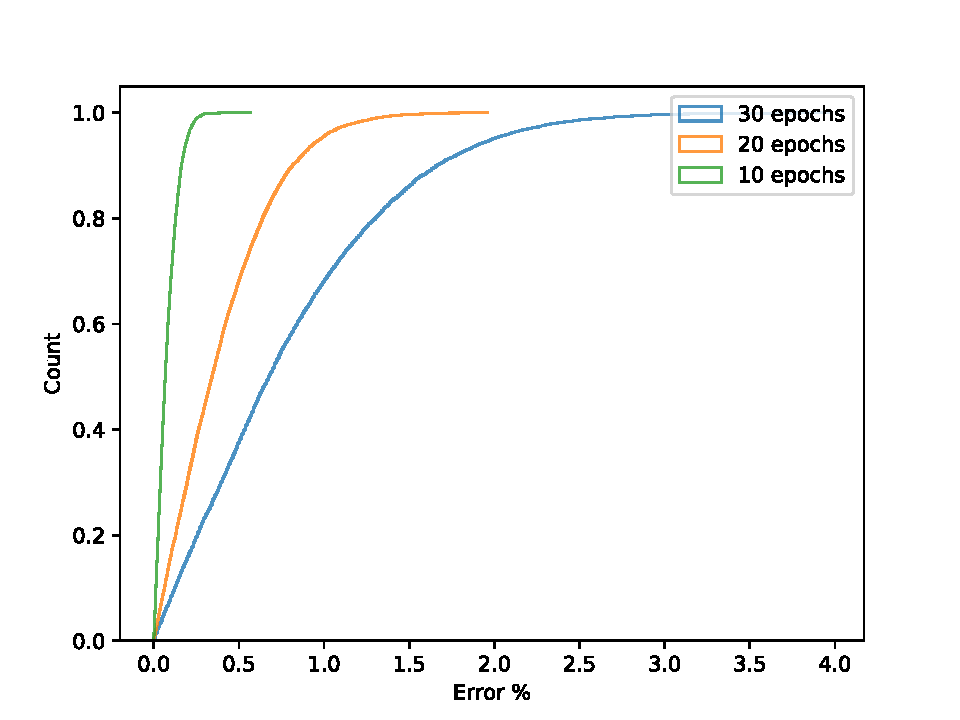
\includegraphics[width=0.9\linewidth]{results/microprofiling_dummy.pdf}
  \end{subfigure}
  \caption{\bf\small Errors in accuracy prediction when using Microprofiling. Accuracy errors are higher when predicting for larger number of epochs, but still within xx\% of the true accuracy.}
  \label{fig:multicam-cities}
\end{figure}

